\section{Approach}
\label{sec:approach}

%Restate the goal/problem. Use Sharon's more descriptive definition of a pattern template.
We aim to develop a method for automatically generating pattern coloring suggestions to facilitate the creative coloring process. One challenge of such a system is that users may or may not have a target coloring style in mind. In addition, aesthetic taste varies across users and can depend on the situation. Thus, an effective color support system should both output a variety of appealing colorings, as well as provide controls to let the user personalize suggestions to her preferred coloring style.

This system should take as input a pattern template and any available user-provided guidelines and output suggested colorings for that pattern template. A pattern template specifies which segments in an image can be colored in, and which segments must map to the same color. For example, an image of a flower on a background may have a template that specifies all petals of the flower must be the same color, and all background segments must be the same color. We refer to the set of segments that map to the same color as a \emph{color group}. Figure~\ref{fig:teaser} shows an example of a pattern template visualized in grayscale, where each lightness level identifies a different color group. This pattern template representation is relatively easy to author from images composed of segments, such as web designs, 3D renderings, and line drawings. In this paper, we focus on 2D graphic design patterns.

To generate attractive pattern colorings, a reasonable first step is to enforce that colors are `compatible' with one another, for some definition of color compatibility. Figure~\ref{fig:ColorCompatOnly} shows several patterns whose colors receive a high score under the color compatibility model of O'Donovan et al.~\shortcite{ODonovan}. While these high-scoring colorings use attractive colors and do exhibit a great degree of diversity, they also display several problems. Some of the patterns have background regions that are oversaturated, giving the impression of being too `loud.' Several foreground regions have insufficient contrast with the pattern background, causing them to blend into the background and become invisible or visually jarring.
%Furthermore, color compatibility is a universal notion: it is not clear how to adapt it to match the style of a particular artist or the preferences of a particular user.

\begin{figure}[htb]
\centering
%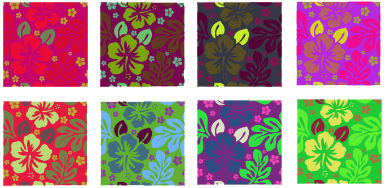
\includegraphics[width=\columnwidth]{figs/colorCompatOnly.png}
\begin{tabular}{cccc}

\includegraphics[width=.2\columnwidth]{figs/colorCompat/r_0_0_3-75}&

\includegraphics[width=.2\columnwidth]{figs/colorCompat/r_0_1_3-32}&

\includegraphics[width=.2\columnwidth]{figs/colorCompat/r_0_2_3-67}&

\includegraphics[width=.2\columnwidth]{figs/colorCompat/r_0_3_3-70}\\
3.75&3.32&3.67&3.70\vspace{0.5em}\\

\includegraphics[width=.2\columnwidth]{figs/colorCompat/r_1_0_3-74}&

\includegraphics[width=.2\columnwidth]{figs/colorCompat/r_1_1_3-42}&

\includegraphics[width=.2\columnwidth]{figs/colorCompat/r_1_2_3-66}&

\includegraphics[width=.2\columnwidth]{figs/colorCompat/r_1_3_3-39}\\
3.74&3.42&3.66&3.39\\
\end{tabular}
\caption{Patterns whose colors receive high scores under the color compatibility model of O'Donovan et al.~\shortcite{ODonovan}. The score assigned by the O'Donovan model is shown beneath each pattern, with a typical pattern receiving a score between 3 and 4. Many results exhibit problems such as adjacent equi-luminant regions and excessively saturated backgrounds.}
\label{fig:ColorCompatOnly}
\end{figure}

To overcome these problems, we can turn to examples of well-colored patterns for help. If we examine color groups that are large, highly connected, and spread across the entire pattern---indicative features of a background---we can see how saturated they are. This knowledge should prevent us from using excessively `loud' background colors. If we look at the typical contrast between adjacent pattern regions, we might find that large foreground regions have high contrast with the background but less contrast with thin borders and outlines. Enforcing these same properties in our own colorings should lead to better results.

Consequently, the approach to pattern coloring we present in this paper is \emph{data-driven}: given a dataset of example patterns, we learn distributions over color properties such as saturation, lightness, and contrast for individual regions and for adjacent regions. We predict these distributions using discriminative spatial features of the pattern, such as the size and shape of different regions.

In the next section, we introduce the dataset of patterns we use for our experiments (Section~\ref{sec:dataset}). Next, we describe the \emph{unary color functions} that we use to predict the color properties of indvidual pattern regions (Section~\ref{sec:unary}), as well the \emph{binary color functions} that predict the properties of adjacent regions (Section~\ref{sec:binary}). While color compatibility alone does not predict good pattern colorings, it helps to enforce global consistency between colors, and our approach makes use of this ability (Section~\ref{sec:colorCompat}).

We then show how these three different types of predictive functions---\emph{unary}, \emph{binary}, and \emph{global}---can be combined into one unified model using the framework of probabilistic factor graphs (Section~\ref{sec:model}). The resulting model is very flexible: we can sample from it to generate a variety of new coloring suggestions, train it on different example sets to capture different coloring styles, and add additional constraints to it to support different usage scenarios (Section~\ref{sec:results}).

%\remark{After pointing out the problems with the images, mention how some simple features (size of region, number of connected components) seem predictive of how colorful it should be. Call out a similar example for an adjacency feature. Mention that compatibility is still important(?) Our approach is to learn to predict these kinds of color properties given these kinds of pattern features, given a dataset of patterns. In the next sections, we'll first describe the dataset we use. Then we'll describe the unary functions we use to predict color properties of pattern regions (cite section), the binary functions we use to predict color properties of adjacent pattern regions (cite section), and our treatment of color compatibility (cite section). We'll then show how all of these different predictive functions can be combined into one unified probabilistic model through the framework of factor graphs. We can automatically tune the relative importance of each function in the model (cite section) and then sample from it to generate coloring suggestions for a given pattern (cite section).
%}
%
%Rather than develop a specialized algorithm for this problem, we exploit the insight that both of these concerns---color harmony and spatial consistency---can be encoded in the extremely general framework of probabilistic factor graphs. In the next sections, we develop a data-driven factor graph model that can be trained on example colored patterns and sampled to generate new coloring suggestions. The factor graph formalism allows us to leverage existing models of color compatibility, to plug in additional coloring constraints in response to available user input, and to capture and inspect the characteristics of desired styles through established machine learning techniques.
